\documentclass[../main.tex]{subfiles}

\begin{document}

The 3D classification problem is specially challenging due to the fact that images need to be classified according to unknown structures. Once these structures have been partially discovered, 3D classification becomes much easier, as particles can be considered to belong to their most similar 3D structure by the means of projection matching.

In this section we aim to describe a new approach that can be used to discover initial solutions without any prior knowledge, except for the 3D alignment of the particles, which implicitly come associated to a consensus volume. A consensus volume is a volume that has been reconstructed with all the particles, disregarding any possible heterogeneity. Thus, it is expected that it expresses a mixture of features from the underlying structures.

Our initial 3D classification approach leverages the fact that particles projected from similar directions should resemble to one another. Thus, grouping particles by their projection angle, should enable us to perform a image classification in 2D. Then, using graph theory, we can relate neighbouring groups, leading to a global classification. An overview of this process is displayed in Figure \ref{fig:4.1:overview}.

\begin{figure}[hbp]
    \centering
    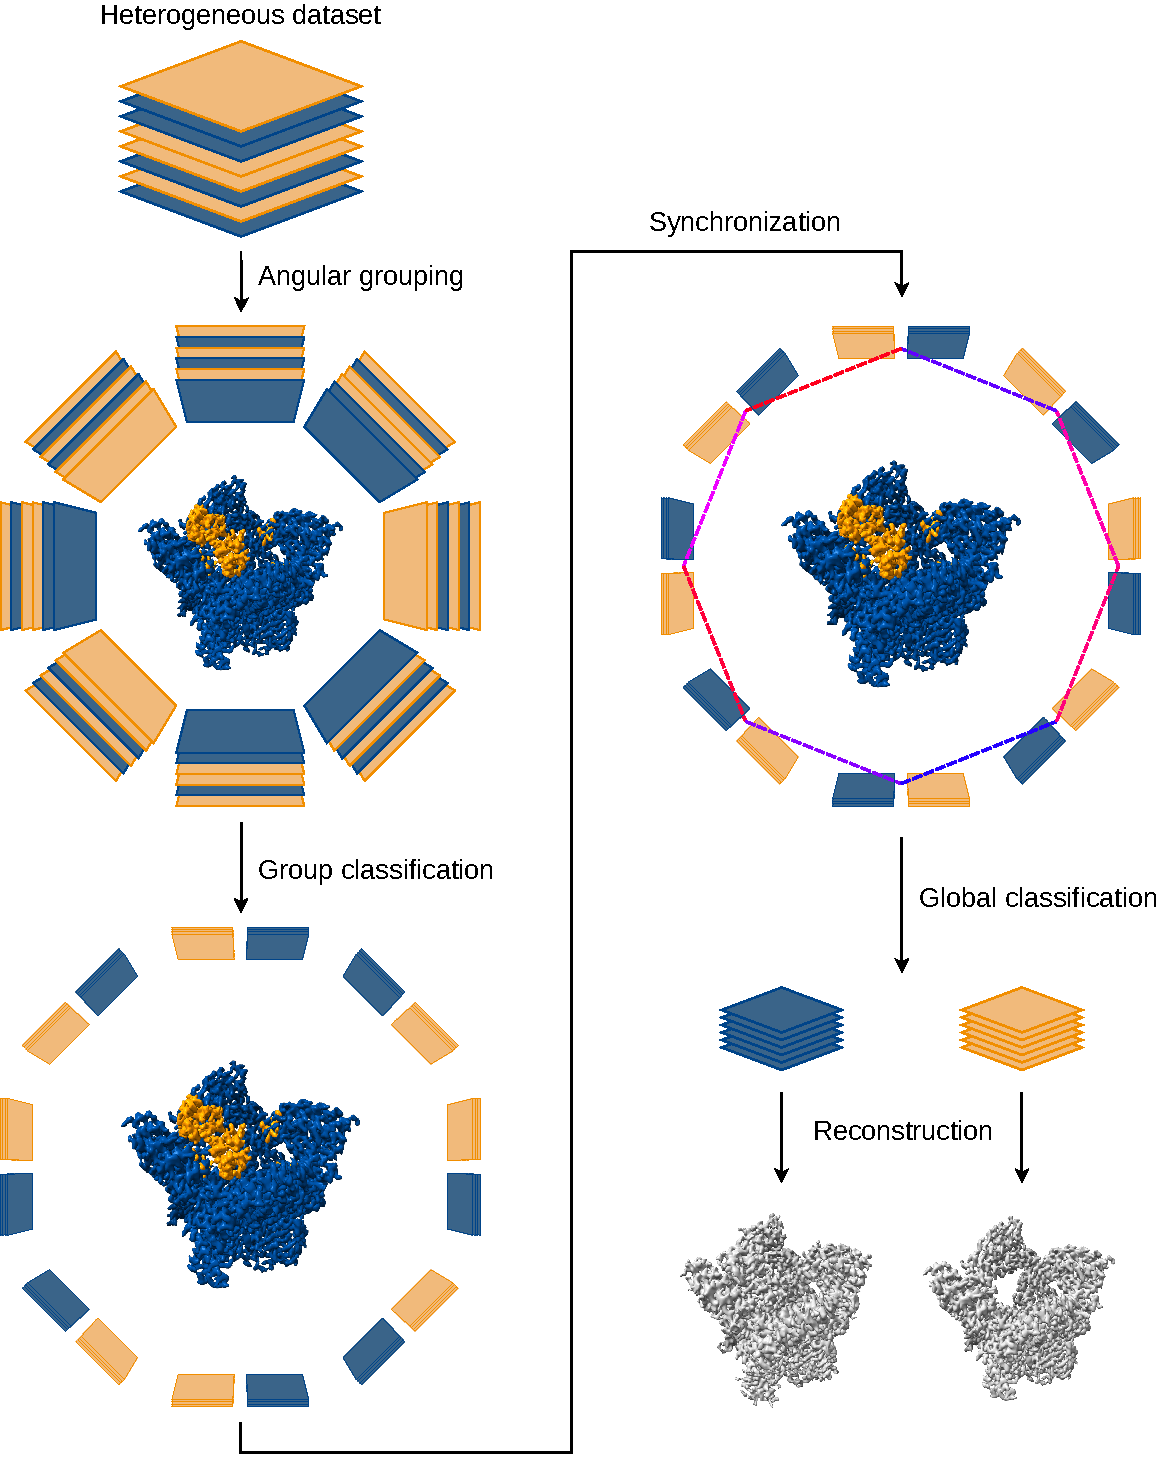
\includegraphics[width=\textwidth]{implementation/overview}
    \caption{Overview of the initial 3D classification algorithm}
    \label{fig:4.1:overview}
\end{figure}

In this early stage, we will ignore the presence of the \gls{ctf} and assume that images have their \glspl{ctf} corrected.

\subsection{Projection grouping}
As a first step, our algorithm groups neighbouring projections, as they are considered to be similar enough and only differ in the structural feature we are interested in. These groups are overlapping, this is, a particle may belong to multiple groups. Indeed, for reasons that will be detailed later, some amount of overlap is mandatory. A example of such a grouping is illustrated in Figure \ref{fig:4.1:cones}.

\begin{figure}[hbp]
    \centering
    \begin{subfigure}[b]{0.6\textwidth}
         \centering
         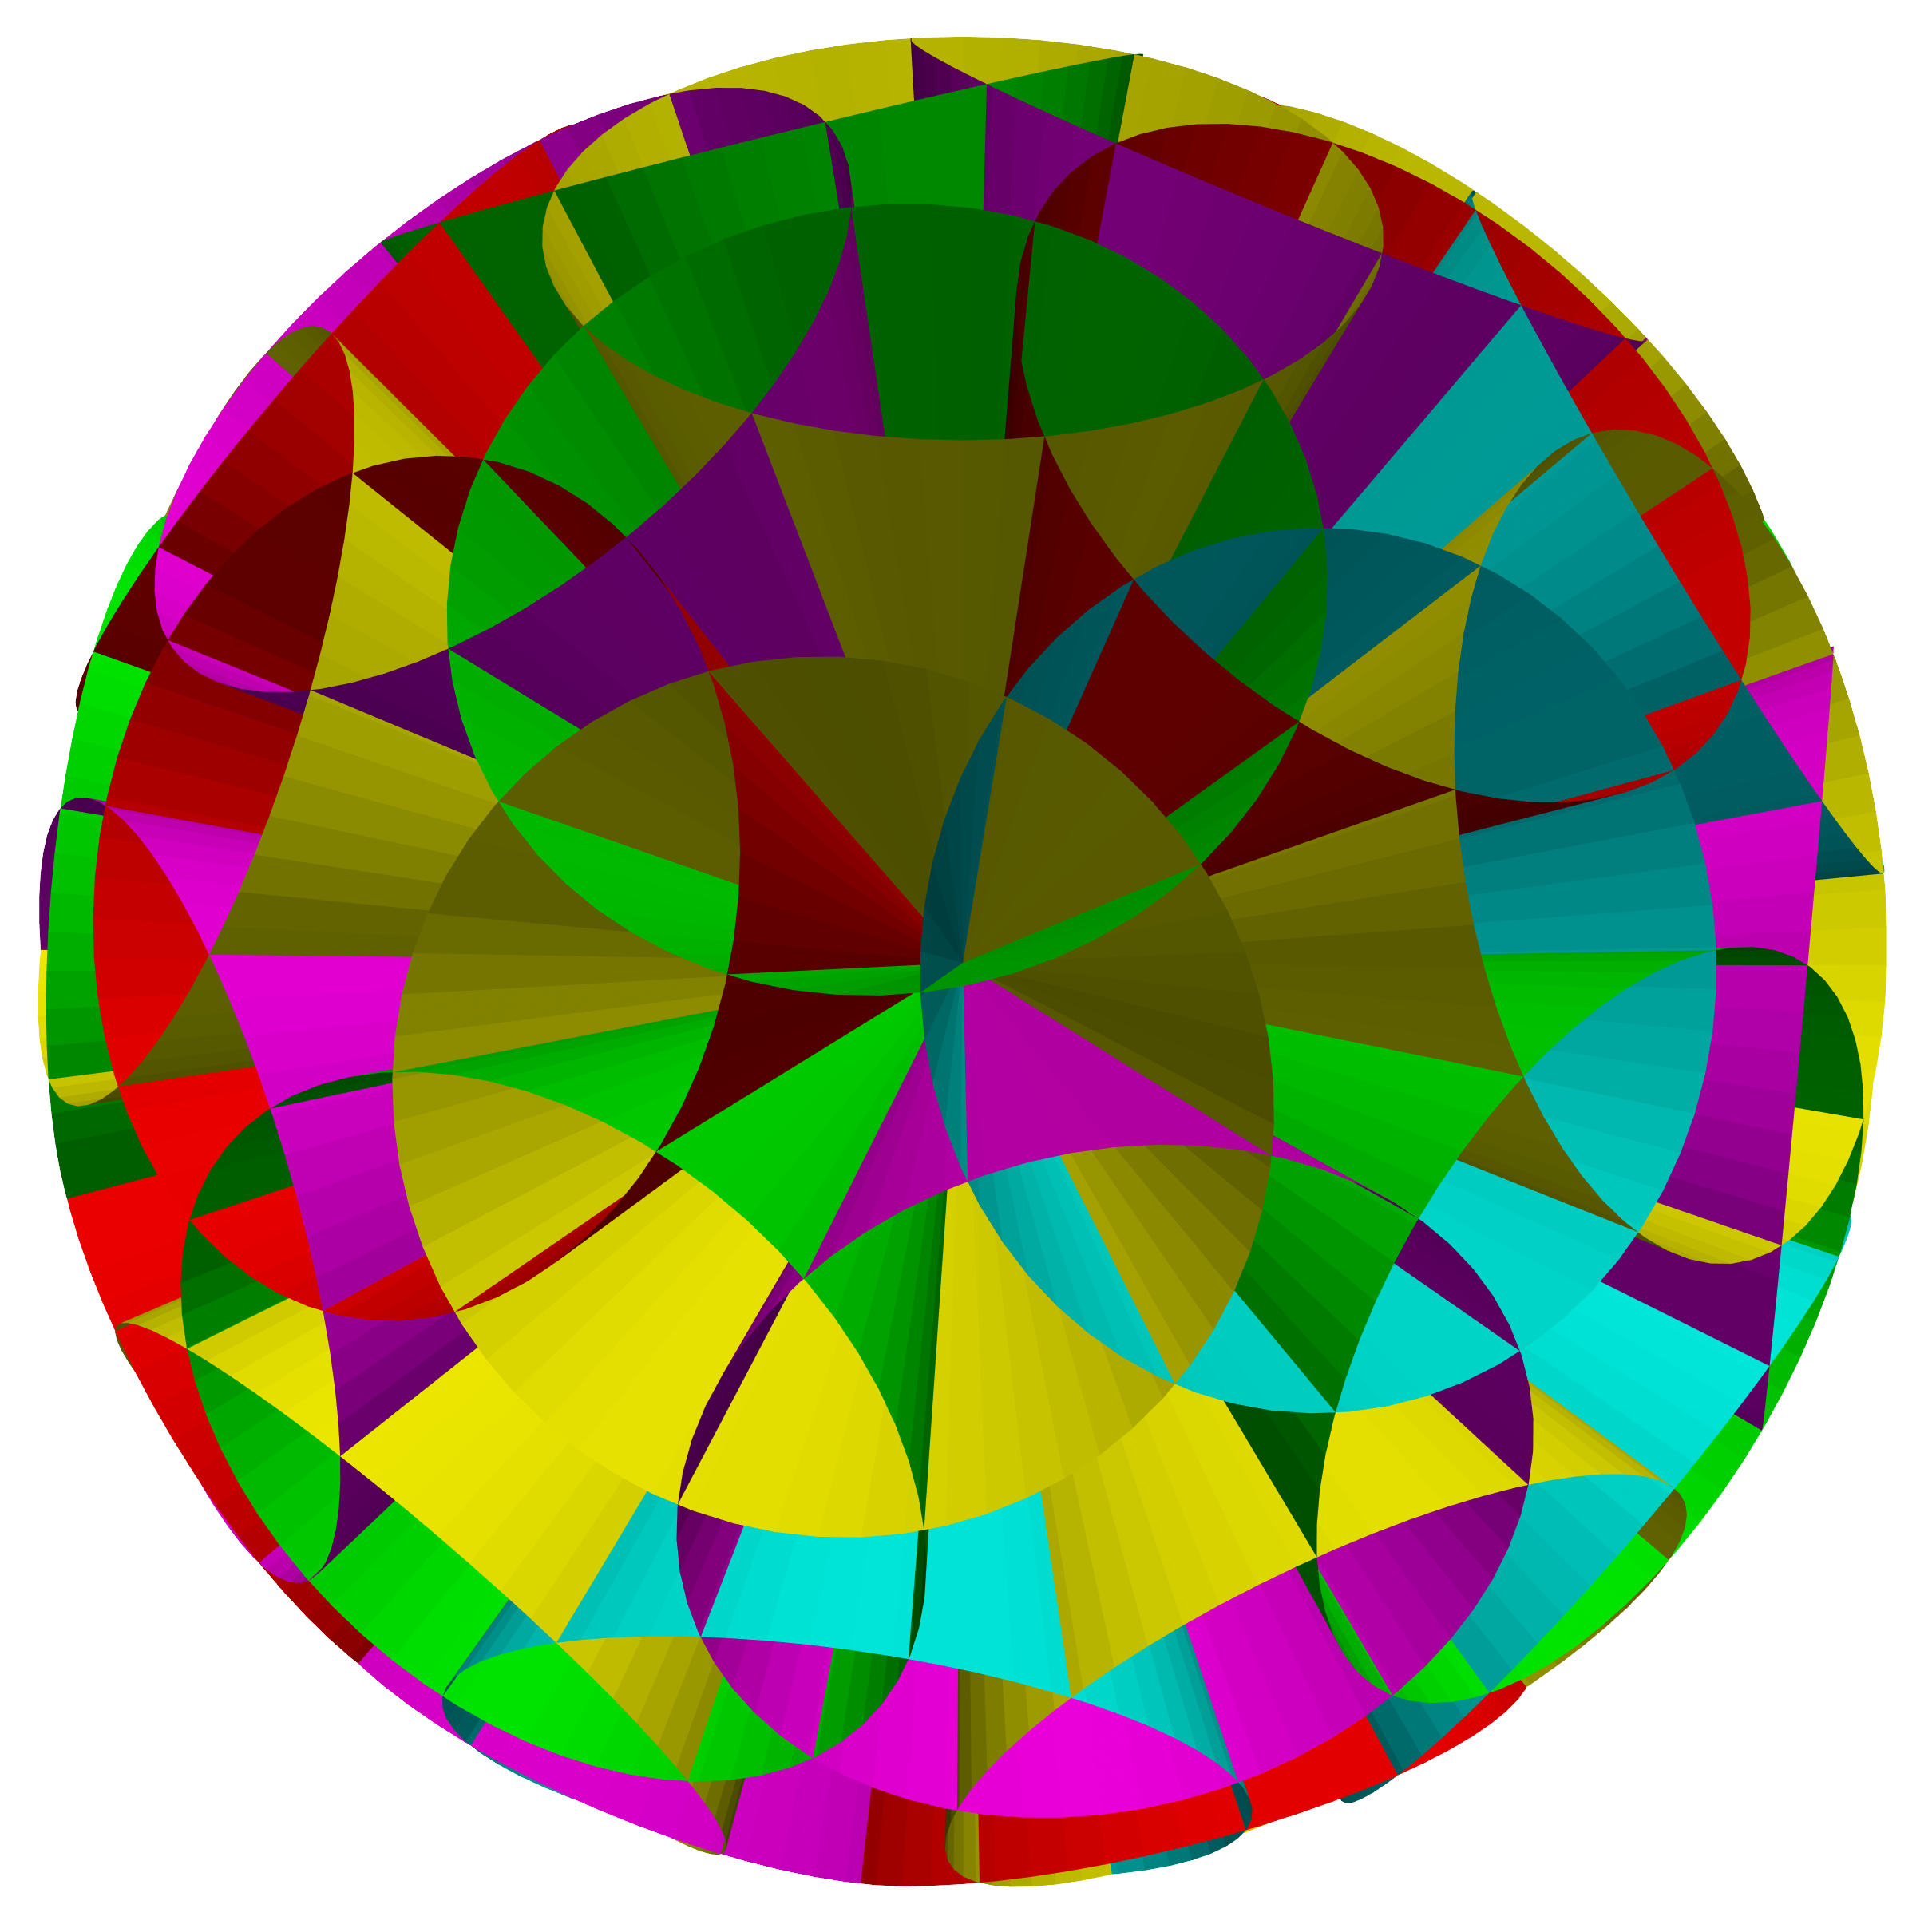
\includegraphics[height=7.5cm]{implementation/cones}
         \caption{Projection sphere divided in overlapping cones}
    \end{subfigure}
    \begin{subfigure}[b]{0.3\textwidth}
         \centering
         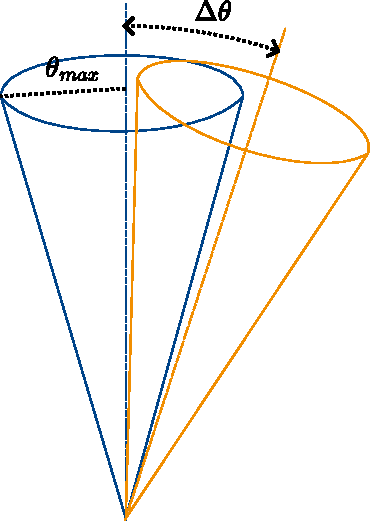
\includegraphics[height=7.5cm]{implementation/theta max}
         \caption{Cone spacing criteria}
    \end{subfigure}
    \caption{Particle grouping with cones}
    \label{fig:4.1:cones}
\end{figure}

Each of these groups has a representative projection direction, which will be named as $\bm{r_i} \in S^2$, where $S^2$ is the unit sphere in $\mathbb{R}^3$. These direction vectors are artificially generated in such a way that they are quasi equally spaced in the unit sphere. These points can be limited to a hemisphere, as projections emanating from antipodes are equivalent, except for a mirror transformation. Additionally, if the protein under study poses symmetry, this can be accounted to further reduce the directions to the unit cell of the corresponding symmetry group.

Regarding the particles themselves, their projection direction is usually represented by a triplet of Euler angles: $(\theta, \phi, \psi)_j$. However, for our purposes, it becomes more handy to represent projection directions of the experimental images with unit vectors $\bm{\gamma_j} \in S^2$. The Euler angles can be easily converted to vector notation using the expression \eqref{eq:4.1:euler_to_vector}:

\begin{equation}\label{eq:4.1:euler_to_vector}
    \bm{\gamma_i} =
    \begin{bmatrix}
        \text{sin}(\text{tilt}_j) \cdot \text{cos}(\text{rot}_j) \\ 
        \text{sin}(\text{tilt}_j) \cdot \text{sin}(\text{rot}_j) \\ 
        \text{cos}(\text{tilt}_j)
    \end{bmatrix}
\end{equation}

At this point, the grouping of projections becomes trivial: A particle is considered to be on a group only if the angle between its projection direction and the representative direction of the group is smaller than some arbitrary threshold $\theta_{max}$:

\begin{equation}
    G_i = \{ j : \text{acos}(\langle \bm{r_i}, \bm{\gamma_j} \rangle) \leq \theta_{max} \}
\end{equation}

$\theta_{max}$ defines the aperture of the cones used for grouping. Thus, it is important to use a value low enough such that the variability induced by the projection direction is negligible compared to the actual variability in the structure. In our experience, a value of $7.5 \si{\degree}$ provides good results. Similarly, the number of groups needs to be sufficient so that these cones overlap. To do so, we are selecting the number of groups so that they are spaced on average by $\Delta\theta \approx \theta_{max}$ as shown in Figure \ref{fig:4.1:cones}. 

\subsection{Classification of neighbouring projections}
In the previous step we have classified images according to their projection direction.  At this point, our intention is to classify the images from each group into two classes that are maximally dissimilar. This process will be applied for each directional group.

\subsubsection{Image alignment}
Before attempting any classification, images need to be aligned to one another. To do so, we will leverage the 3D alignment estimation provided by the preceding steps in the \gls{spa} image processing pipeline. The three possible in-plane transformations are represented in Figure \ref{fig:4.1:inplane}.

\begin{figure}[hbp]
    \centering
    
\includegraphics[width=.4\textwidth]{implementation/inplane}
    \caption{In-plane transformation of the particles}
    \label{fig:4.1:inplane}
\end{figure}

First, the center offset of the particles accounted by displacing them by their shift estimate $(\delta_x, \delta_y)$ in the opposite direction. This ensures that the particle is centered in the image frame. 

Secondly, the in-plane rotation of the particles is corrected. To do so, the Euler angle estimates are converted to quaternion space. Then, the quaternion $\bm{Q_j} = (\bm{v_j}, w_j) = (\bm{u_j} \cdot \sin\theta_j, \cos\theta_j)$ is projected onto the $\bm{r_i}$ axis using the expression \eqref{eq:4.1:twist}. This expression was derived from the twist-swing\cite{chou2018} decomposition, which describes a quaternion with two components: a rotation around a certain axis and the residual part. In this case, we are only interested in the rotation around the projection direction.

\begin{equation}\label{eq:4.1:twist}
    \hat{\psi} = \text{atan2}(\langle \bm{v_j}, \bm{r_i} \rangle, w)
\end{equation}

Note that the $\psi$ component of the Euler angles also expresses the in-plane rotation. However, due to the fact that we are combining images with (slightly) different projection angles, $\hat{\psi}$ leads to a more precise in-plane alignment.

In practice, both of the alignment operations (rotation and shift) are performed at once with an affine matrix transformation. This matrix is shown in Equation \eqref{eq:4.1:affine}. Note that the shift is applied before the rotation, so the rotation is also applied to the shift vector.

\begin{equation}\label{eq:4.1:affine}
    M =
    \begin{bmatrix}
        \cos \hat{\psi} & -\sin \hat{\psi} & 0\\
        \sin \hat{\psi} & \cos \hat{\psi} & 0\\
        0 & 0 & 1\\
    \end{bmatrix}
    \cdot
    \begin{bmatrix}
        1 & 0 & \delta_x\\
        0 & 1 & \delta_y\\
        0 & 0 & 1\\
    \end{bmatrix}
    =
    \begin{bmatrix}
        \cos \hat{\psi} & -\sin \hat{\psi} & \cos \hat{\psi} \cdot \delta_x - \sin \hat{\psi} \cdot \delta_y\\
        \sin \hat{\psi} & \cos \hat{\psi} & \sin \hat{\psi} \cdot \delta_x + \cos \hat{\psi} \cdot \delta_y\\
        0 & 0 & 1\\
    \end{bmatrix}
\end{equation}

\subsubsection{Image classification}
Once all the particles of a directional group are aligned to one another, a classification is attempted. To do so, we have used \gls{pca}, a popular dimensionality reduction technique\cite{kurita2019}. In short terms, \gls{pca} describes a set of multidimensional points in an orthogonal basis where its components are not correlated. Moreover, components of the basis are ordered by the variance they capture\cite{karamizadeh2013}.

On our approach, we consider a lexicographically ordered version of the image (pixels layed out as a 1D vector), so that \gls{pca} can be applied to them. This ordering is performed withing a mask, so that the classification can focused on a \gls{roi}. This mask is generated by projecting the input 3D mask in the reference direction.

This \gls{pca} procedure is applied in each group to an aligned stack of particles as shown in Figure \ref{fig:4.1:eigenimage}. Assuming that the primary source of variability across images is the heterogeneity, the first eigen-image will be representative of this heterogeneity.

\begin{figure}[hbp]
    \centering
    
\includegraphics[width=.8\textwidth]{implementation/PCA}
    \caption{Eigen-image computation process}
    \label{fig:4.1:eigenimage}
\end{figure}

In our implementation, we use \texttt{pytorch}\cite{paszke2019} to perform the \gls{pca} analysis and obtain the first eigen-image. Then, the eigen-image can be used as a projection basis for the images. This allows to order particles according to their projection value. Indeed, this can be interpreted as an interpolation weight between two classes that are maximally dissimilar, $C_+$ and $C_-$.

\begin{equation}\label{eq:4.1:pca_projection}
    \rho_i = \langle \bm{u_1}, \bm{x_i} \rangle
\end{equation}

where $\bm{u_1}$ is the first principal component (largest eigenvalue) and $\bm{x_i}$ is the vector representation of a particle.

We will assume that \gls{pca} projection values of follow Gaussian distributions $C_+ \sim \mathcal{N}(\mu_+, \sigma_+^2)$ and $C_- \sim \mathcal{N}(\mu_-, \sigma_-^2)$. Thus, using the projection values we can attempt a classification by fitting a \gls{gmm} of two components to their histogram. To avoid numerical stability issues, we enforce the same variance for both \gls{gmm} components ($\sigma_+^2 = \sigma_-^2$). Consequently, each component of the \gls{gmm} can be used to estimate the likelihood of their corresponding class. An example of such a fitting is displayed in Figure \ref{fig:4.1:gmm}.

\begin{figure}[hbp]
    \centering
    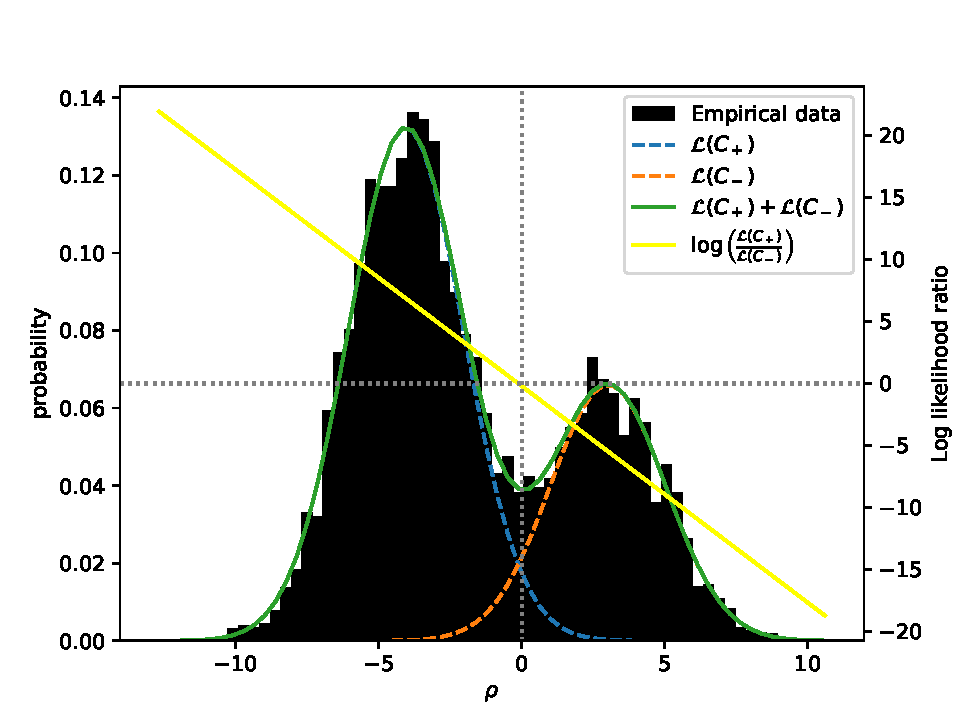
\includegraphics[width=.8\textwidth]{implementation/gmm}
    \caption{Example of a Gaussian Mixture Model of two components}
    \label{fig:4.1:gmm}
\end{figure}

Computing the log likelihood ratio of the components, we can rank particles according to the class they most likely belong to. In other words, log likelihood ratio's sign determines which of the classes is more probable, while its magnitude reflects the certainty. This ratio is also plotted in Figure \ref{fig:4.1:gmm}.

\begin{equation}\label{fig:4.1:likelihood}
    \text{log}\ \Lambda(\rho) = \text{log}\ \frac{\mathcal{L}(C_+\ |\ \rho)}{\mathcal{L}(C_-\ |\ \rho)}
\end{equation}

We will name the log likelihood ratio of a given particle as $\lambda_i$:

\begin{equation}
    \lambda_i = \text{log}\ \Lambda(\rho_i) 
\end{equation}

\subsection{Directional class synchronization}
In the previous step we have established two classes for each of the directional groups. It is expected that these classifications have been performed according to the heterogeneity we are interested in. However, this does not mean that classes match across groups. In fact, \gls{pca} has two equally valid solutions for each axis, which are opposite to one another. Similarly, the \gls{gmm} fitting is arbitrary. Thus, class ordering is not deterministic. In other words, $C_+$ in one group may correspond to $C_-$ in another group and vice versa.

Consequently, a synchronization of classes across directional groups is required. That is why cones need to overlap. Doing so, we can make use of common particles to evaluate if a given pair of adjacent groups have equal or opposite classifications. 

The first step to perform this synchronisation is to find the common particles by computing the set intersection of adjacent groups:
\begin{equation}\label{eq:4.1:intersection}
    I_{ij} = G_i \cap G_j
\end{equation}

The dot product of the log likelihood ratios of common particles in each group can be used as a similarity metric to compare their classifications. Positive values indicate that the classifications are aligned. Accordingly, negative values point that the classes are swapped. 

\begin{equation}\label{eq:4.1:weights}
    w_{ij} = \sum_{p \in I_{ij}} \lambda_{ip} \cdot \lambda_{jp}
\end{equation}

At this point we want to maximize the compatibility of all directions by flipping the classifications of a given set of groups. This swapping of classes translates into applying a negative sign to all their log likelihood ratios. According to the expression \eqref{eq:4.1:weights}, this would also result in the application of this negative sign to all the weights related to these groups. 

Thus, we can express our synchronization problem as the quadratic binary optimisation problem posed in equation \eqref{eq:4.1:optimisation}. This is, we want to maximise the total compatibility by flipping some classifications.

\begin{equation}\label{eq:4.1:optimisation}
\begin{aligned}
    & \max_{\bm{\sigma}} f(\bm{\sigma}) = \sum_{i, j} w_{ij} \cdot \sigma_i \cdot \sigma_j = \bm{\sigma}^T W \bm{\sigma}\\
    \text{subject to}\\
    & \sigma_i \in \{-1, +1\} \Leftrightarrow \sigma_i^2 = 1
\end{aligned}
\end{equation}

where the sign of $\sigma_i$ relates to a group being swapped or not. 

\subsubsection{Analogy with magnetic dipoles}
Although this optimisation problem may look naive, it is not trivial to solve, as it cannot be approached with Lagrange multipliers. Similar cases to this problem also appear in nature, as is the case of the Hamiltonian of the Ising Model\cite{kennedy2008}.

The Ising Model describes the behaviour of a network of magnetic dipoles where these may freely flip their polarity. The Hamiltonian of the model represents the energy of the system\cite{kennedy2008}. As in many cases in nature, the energy of a system tends to be minimal, and the Ising Model is not an exception to this rule. Thus, the Ising Model will be on a stable state only if its Hamiltonian is minimal. The expression for Hamiltonian of the Ising Model without external interactions is provided hereafter:

\begin{equation}\label{eq:4.1:ising}
\begin{aligned}
    & H(\bm{\sigma}) = -\sum_{i, j} J_{ij} \cdot \sigma_i \cdot \sigma_j\\
    & \sigma_i \in \{-1, +1\}
\end{aligned}
\end{equation}

where $J_{ij}$ represents the magnetic interaction between each pair of dipoles. When $J_{ij} > 0$ the interaction is ferromagnetic (magnet polarities to align) and when $J_{ij} < 0$ the interaction is anti-ferromagnetic (magnet polarities tend to oppose). $\sigma_i$ represents the spin of each of the magnetic dipoles in the system. This will help us establish a classification-magnet metaphor.

Except for the minus sign, the expression \eqref{eq:4.1:ising} is equal to our objective function detailed in \eqref{eq:4.1:optimisation}. Indeed, due to this duality, the minimisation of the energy in the Ising Model corresponds to the maximisation of our objective function. Therefore, solutions to the Ising Model also serve as solutions for our problem. 

One of the most common ways to approach the Ising Model problem is by finding the maximum cut of the graph defined by the weighted adjacency matrix $\bm{A} = -\bm{J}$, which in our case corresponds to the similarity matrix $\bm{W}$. Once the graph has been bi-partitioned using the maximum cut criteria, magnets (or classes) of one partition are flipped to minimize energy (or maximize compatibility)\cite{kennedy2008}.

An example of a graph of direction similarities is detailed in Figure \ref{fig:4.1:graph}, where the edge colours represent the similarity metric between adjacent directions. The vertices are positioned in $\bm{\gamma_i}$, so that the graph appears to be embedded in the projection sphere.

\begin{figure}[hbp]
    \centering
    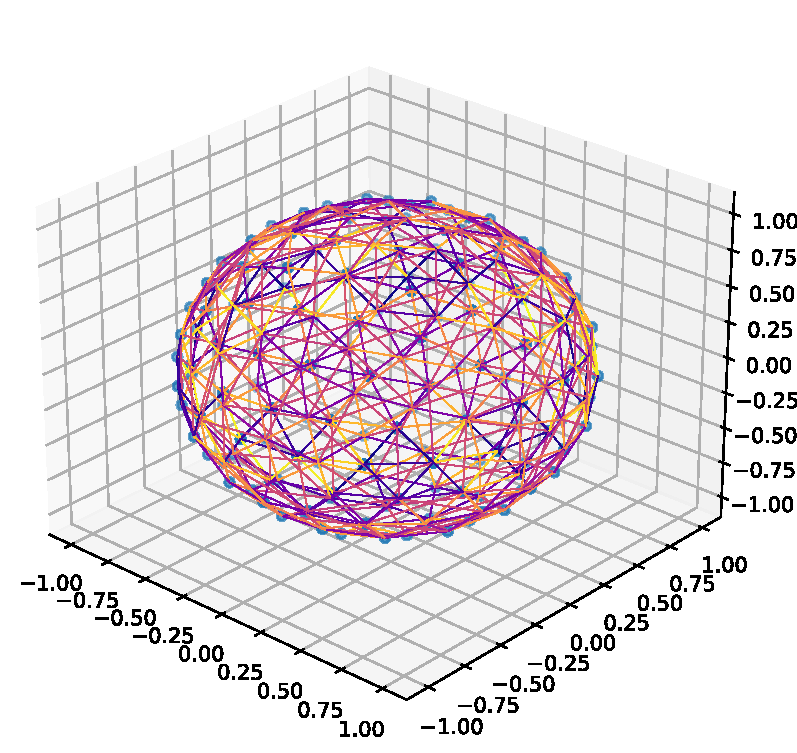
\includegraphics[width=.7\textwidth]{implementation/3d graph}
    \caption{Graph embedded on the projection sphere}
    \label{fig:4.1:graph}
\end{figure}

\subsubsection{Graph maximum cut algorithm using SDP}
Until this point we have only shifted our optimisation problem into other domains, without giving any concrete solution to it. Nevertheless, we have reasoned that our problem directly maps to the graph maximum cut problem.

A graph cut is a partition of the graph into two disjoint sets of vertices (no edges connecting the two subsets). Thus, the the graph cut size is the sum of the edges that need to be removed to obtain a disjoint bi-partition. Considering the former definition, the graph maximum cut is defined as ``A cut whose size is at least the size of any other cut''\cite{sudakov2005}. However, similar to the previous analogies, this problem is not easy to solve, as it is deemed NP-Hard\cite{chan2014}. Luckily, numerous heuristic approaches exist that provide reasonably bounded solutions.

In our case, we have decided to use an approach based on \gls{sdp}. This approximation is guaranteed to find a solution that is at least $87 \si{\percent}$ accurate while also being computationally efficient\cite{kemal2008}.

The \gls{sdp} approach involves relaxing $\sigma_i \in \{-1, +1\}$ to $\bm{x_i} \in S^{N-1}$ where $S^{N-1}$ is the unit sphere in $\mathbb{R}^N$. This allows us to define the matrix $\bm{X}$ of pairwise dot products:

\begin{equation}
    X_{ij} = \langle \bm{x_i}, \bm{x_j} \rangle
\end{equation}

Due to the commutative property of the inner product, we can deduce that $\bm{X}$ must be symmetric. Moreover, all its diagonal values must be 1, as these involve the dot product of a unit vector with itself. Last but not least, this matrix is also guaranteed to be positive semi-definite\cite{kemal2008}. Considering all these constraints, we can pose the \gls{sdp} problem shown in Equation \eqref{eq:4.1:relaxation}. The greatest benefit of this formulation is that there are \gls{sdp} solvers that run in polynomial time (as opposed to the binary optimisation problem which was NP-Hard).

\begin{equation}\label{eq:4.1:relaxation}
\begin{aligned}
    & \min_{\bm{X}} f(\bm{X}) = \sum_{i,j} a_{ij}X_{ij}\\
    \text{subject to}\\
    & \bm{X} = \bm{X}^T\\
    & X_{ii} = 1\\
    & \bm{X} \succeq 0
\end{aligned}
\end{equation}

In our implementation, we use \texttt{cvxpy}\cite{agrawal2018}\cite{diamond2016} package to solve this \gls{sdp} problem. To get back the values of $\bm{x_i}$ from $\bm{X}$ we use matrix square root function available in \texttt{scipy}\cite{virtanen2020}. Finally, we undo the relaxation to extract $\sigma_i$ from $\bm{x_i}$\cite{kemal2008}:

\begin{equation}
    \sigma_i = \text{sign}(\langle \bm{v}, \bm{x_i} \rangle)
\end{equation}

where $\bm{v}$ is a random vector in $S^{N-1}$.

\subsection{Global classification}
As a final step, we combine the information gathered from all the 2D classifications to obtain a 3D classification of the particles. To do so, once all the 2D classifications have been synchronized to one another, all the log likelihood ratios of a given particle are averaged (remember that a particle may belong to several directional groups). Recalling that the sign of the log likelihood ratio represents the class, this sign is used to assign the 3D class of the particle.

After bi-partitioning the particle set according to their 3D class, a volume is homogeneously reconstructed for each of the 3D classes. This is done though the \texttt{xmipp\_reconstruct\_fourier} program, which was already implemented in the Xmipp suite\cite{strelak2019}.

\begin{figure}
    \centering
    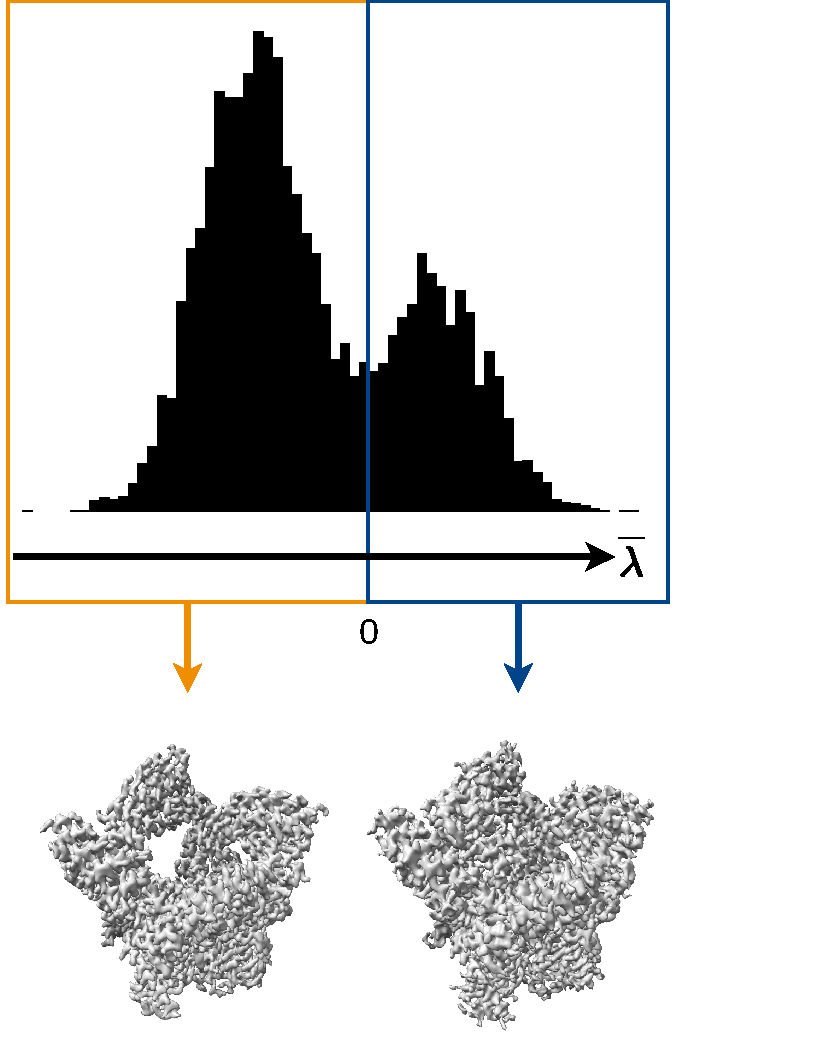
\includegraphics[width=.6\textwidth]{implementation/global classification}
    \caption{Global classification}
    \label{fig:4.1:global}
\end{figure}

\end{document}
